\pagestyle{fancy}

\graphicspath{ {Figures/Chapter3_BeamMatterInteraction/} }

The response characteristics of detection instruments employed during this desis depend on the interaction of charged particles with the sensitive elements of the detectors. In order to correctly interpret the measurements, it is fundamental to understand the various types of interactions between charged particles and matter. Many general reference works are available concerning this broad topic. For example, \parencite*[]{ref:Knoll}, \parencite*[]{ref:Evans} or \parencite*[]{ref:avernier} are very good references. This chapter will introduce only the theoretical concepts necessary for the comprehension of the latter chapters. 

\section{Particle matter interaction.}

The interactions that we will fixate on are primarily those related to Coulomb forces between the incident charged particle and the electrons and nuclei of the detector material. These include ionization, excitation, Bremsstrahlung and Cherenkov radiation. During these interactions, the incident charged particle loses its energy and it can be deflected from its original path. 

In the case of heavy charged particles, that is, particles whose rest mass is large compared with that of the atomic electron, inelastic collisions with atomic electrons are usually the predominant interaction mechanism. In such encounters, the electrons in the medium might experience a transition to an excited state (excitation) or to an unbound state (ionization). Since heavy particles are rarely deflected while traveling near an atomic nucleus, Bremsstrahlung production will be considered to be inconsequential. 

Cherenkov radiation will also be neglected as the conditions for its observation will never be reached in the casuistics of this thesis \parencite*[]{ref:Cherenkov}. For this reason, for the rest of the chapter, we will focus our attention solely to energy losses due to ionization and excitation processes. 

\section{Energy Loss: The Bethe Bloch Formula}
\label{sec:Bethe}

Stopping power is the parameter used to describe the gradual loss of energy of a charged particle as it penetrates into a medium. For a given heavy incident particle and target, this energy loss is very dependent on the particle velocity. In moderately relativistic energy ranges ($10$ - $10^6$ \si[]{\mega \electronvolt}/amu), the electrostatic stopping power is well defined by the Bethe Bloch theory \parencite[]{ref:Bethe}. 

\begin{equation}
    - \left< \frac{dE}{dx} \right> = Kz^2_e\frac{Z}{A}\frac{1}{\beta^2}\left[ \frac{1}{2} ln \left( \frac{2m_e c^2 \beta^2 \gamma^2 T_{max}}{I^2}\right) -\beta^2 - \frac{\delta\left(\beta \gamma\right)}{2} \right]
    \label{eq:bethe}
\end{equation}

With the symbol and parameter definitions given in table \ref{tab:ParBethe}. The units for the Stopping power are \si[]{\mega \electronvolt}/amu. The mean excitation energy is very dependent on the material, and it can vary from a few \si[]{\electronvolt} for materials with low Z to a hundred of \si[]{\electronvolt} for materials with high Z. A good approximation can be formulated as follows \parencite*[][]{ref:IonizationEne}:

\begin{equation}
    I \left[ eV \right] = 10 \cdot Z 
    \label{eq:ionizationEnergy}
\end{equation}

The maximum energy that can be transferred to a target electron in a single head-on collision is described by $T_{max}$, and can be approximated by the following formula \parencite*[][]{ref:TmaxFormula}: 

\begin{equation}
    T_{max} = \frac{2m_e c^2 \beta^2 \gamma^2}{1+\frac{\gamma m_e c^2}{M c^2}+\left( \frac{m_e c^2}{M c^2} \right)^2}
    \label{eq:tmax}
\end{equation}

Finally, $\delta (\beta \gamma)$ is a parametrized density correction factor necessary for highly relativistic particles \parencite*[][]{ref:Bethe}, its units are $MeV cm^2 g^{-1}$. It is important to notice that the energy deposited will very much depend on the characteristics of the incident particle as well as the absorber $\left( -\left< \frac{dE}{dx} \right> \propto \frac{Z}{A}  \right)$. 

\begin{table}[h!]
    \centering
    \begin{tabular}{ccc}
    \hline
    \textbf{Symbol}                  & \textbf{Definition}                  & \textbf{Units or Value}                                               \\ \hline
    $N_A$                      & Avogadro's Number           & $6.0221415(10)\cdot10^23$ $mol^{-1}$ \\
    $z_e$                      & Charge of incident particle &                                                              \\
    Z                       & Atomic number of absorber   &                                                              \\
    A                       & Mass Number of absorber     &                                                              \\
    I                       & Mean excitation energy      & eV                                                           \\
    $\beta \gamma$              & Relativistic parameters     &                                                              \\
    $m_e c^2$ & Electron Mass $\cdot$ $c^2$          & 0.510998918(44) MeV                                          \\
    $r_e$                      & Clasical Electron Radius    & 2.8179403250(28) fm                                          \\
    M                       & Incident Particle Mass      & $MeV/c^2$\\
    
    K/A                     & $4 \pi N_A r_e^2 m_e c^2/A$ & 0.307075 $MeV g^{-1} cm^2$  \\
     $\alpha$ & fine-structure constant & 1/137 \\ 
     \hline
    \end{tabular}
    \caption{Summary of variables used in this section.}
    \label{tab:ParBethe}
\end{table}


 Figure \ref{fig:EneDep} shows as an example, a comparison between energy deposition in thin target materials. In this particular case of thin target detectors, the energy deposition increases until reaching a maximum, after which it starts decreasing. From the image, we can observe that the energy deposited in graphite and copper is larger, due to their smaller mass number. Tungsten, gold and lead present smaller energy deposition values, and are similar to one another, due to their close atomic mass number. 

 \begin{figure}[h]
    \centering
    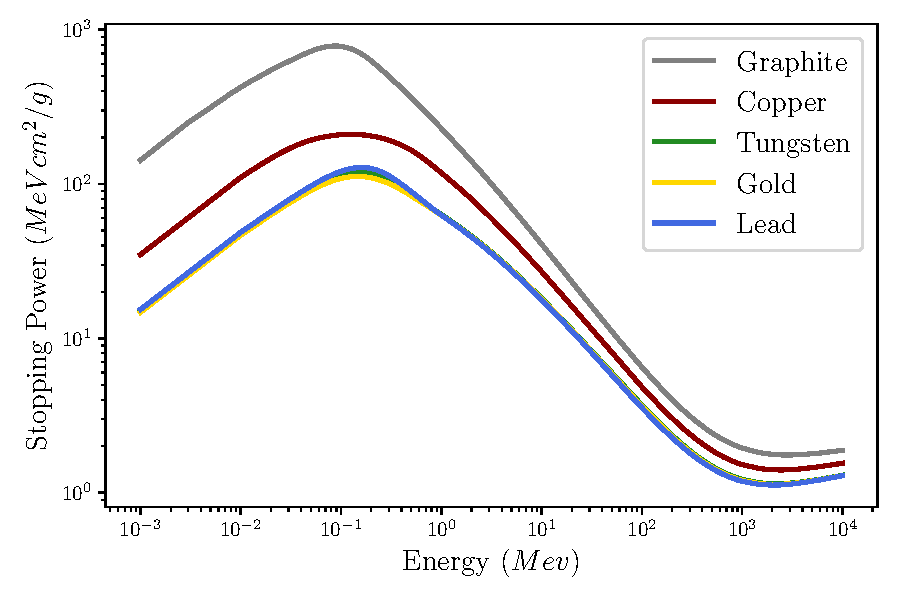
\includegraphics[width=0.7\columnwidth]{EdepMetal/EneDepMetal.pdf}
    \caption{Stopping powrer of protons in thin foils of different materials, as a function of incident particle energy. From \parencite*[][]{ref:NIST}.}
    \label{fig:EneDep}
\end{figure}

\section{Energy Loss in Mixtures and Compounds.}

As a first approximation, one can consider a compound to be made up of very thin layers of pure elements in the right proportion. That is: 

 \begin{equation}
    \frac{dE}{dx} =  \sum w_j \left.\frac{dE}{dx} \right\vert_j
 \end{equation}

Where $\left. \frac{dE}{dx}\right\vert_j$  is the energy loss in the j-th compound. However, it is important to remember that this is an approximation. The values of I and $\delta (\beta\gamma)$ are not perfectly represented by this addition method. More accurate values can be found in \parencite*[][]{ref:compound1} and \parencite*[][]{ref:compound2}, which include measured coefficients for nearly 200 mixtures and compounds. 

\section{Electrons Energy Loss}

For light particles such as electrons, bremsstrahlung losses are not negligible and can become dominant for energies above a few tens of \si[]{\mega\electronvolt}. One can define the critical energy $(E_c)$ as the point where the loss rates by Ionization and bremsstrahlung are the same \parencite*[][]{ref:EleCricEne}. 

\begin{equation}
    E_c = \frac{800}{Z + 1.2}
    \label{eq:ec}
\end{equation}

% When the energy of the incident particle is higher than the critical energy, one can define the energy loss by Bremsstrahlung as follows: 

% \begin{equation}
%     - \left< \frac{dE}{dx} \right> = \frac{E}{X_0}
%     \label{ref:edepElectron}
% \end{equation}

% With`$X_{0}$ being the radiation lenght, and defined as: 

% \begin{equation}
%     \frac{1}{X_0} = 4\alpha r^{2}_{e} n_{at} \left( Z^{2} \left[L_{rad}-f(Z)\right] + Z L^{'}_{rad}\right)
% \end{equation}

% \begin{equation}
%     L_{rad}(Z) = ln(184.15/Z^{1/3})
% \end{equation}

% \begin{equation}
%     L'_{rad} = ln (1194/Z^{2/3})
% \end{equation}

% Here, $n_at$ is the number of atoms per volume ($N_{av}\rho/A$). f(Z) is the coulomb correction function. 

Figure \ref{fig:BremssVSion} shows the stopping power of electrons in a thin tungsten target. From this figure we can see how in this case radiative losses become relevant after incident energies $\> 10 $\si[]{\mega\electronvolt}. This quantity is in agreement with equation \ref{eq:ec}.  

Due to the energy ranges and particles treated during this thesis, bremsstrahlung losses will not be considered as we will always remain under the critical energy regime. Some more information about how to model the energy losses due to this process can be found in \parencite*[][]{ref:BremstutorialG4}. 

\begin{figure}[h]
    \centering
    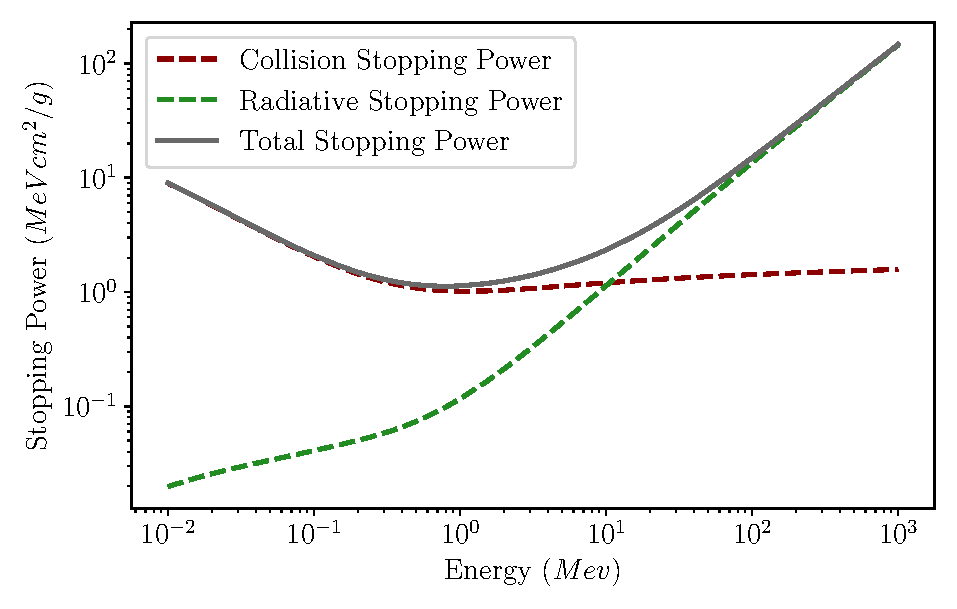
\includegraphics[width=0.7\columnwidth]{Electron_Edep/ElectronEdep.pdf}
    \caption{Stopping power of electrons in a thing tugsten foil, as a function of incident particle energy. From \parencite*[][]{ref:NIST}}
    \label{fig:BremssVSion}
\end{figure}

\section{Multiple scattering}

During the passage of the charged particle through the material, not only changes in the energy will occur, but also deflections from its original path. Most of these deflections occur due to Coulomb scattering with the atomic nucleus (Rutherford-type collisions). These collisions will result in small angular deflections ( if $m_{nucleus} >> m_{particle}$ ). Figure \ref{fig:PartScattering} shows a schematic representation of this process. 

\begin{figure}[h]
    \centering
    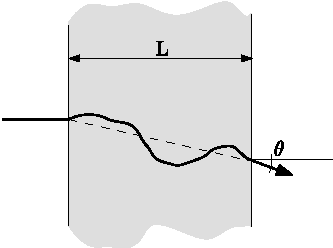
\includegraphics[width=0.4\columnwidth]{MultipleCoulombScat/MultipleScat.pdf}
    \caption{Schematic representation of multiple coulomb scattering.}
    \label{fig:PartScattering}
\end{figure}


The thicker the absorber and the larger its atomic number Z, the greater the likelihood that the incident particle will suffer multiple scatting events. Generally, 20 collisions are deemed sufficient to consider multiple scattering. For a sufficiently thick absorber, the mean number of successive encounters rises to a value that permits a statistical treatment of the problem. This is well represented by the theory of Moliere \parencite*[][]{ref:Moliere}, which assumes that after a distance L traveled through the material, the angular distribution of the particles with respect to their initial direction is Gaussian in shape and centered around the direction of the incident particles. This assumes that the deflection angle will be very small ($\theta \leq 10 \deg $). In these conditions, the mean square angle of such a Gaussian distribution can be calculated as follows: 


\begin{equation}
    \theta_0 = \frac{13.6 MeV}{\beta p c} z \sqrt{\frac{l}{X_0}}\left[ 1+0.038ln\left(\frac{l}{X_0}\right)\right] 
    \label{eq:multscat}
\end{equation}

Here $p,\beta c $ and z are the momentum, velocity and charge number of the incident particle and $l/X_0$ is the thickness of the medium measured in radiation lengths $X_0$, discussed in the following section. Experimental measurements show excellent agreement with the Gaussian distribution at small angles, and as expected, start differing at larger angles. This divergence can be explained due to the higher probability of close encounters which result in larger scattering angles. 

\section{Electron Back-Scattering}
\label{sec:BS}
It is very difficult to study any theory of multiple scattering for incident light particles such as electrons, due to the large number of scattering processes, not only by the atomic nuclei but also by the other electrons in the medium \parencite*[][]{ref:MultipleElec1} Equation \ref{eq:multscat} would need some corrections to properly describe the multiple scattering suffered by this light incident particle \parencite*[][]{ref:MultipleElec2}

\begin{figure}[h]
    \centering
    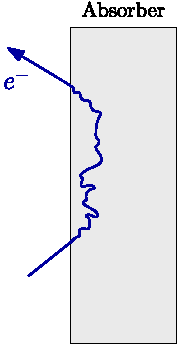
\includegraphics[width=0.25\columnwidth]{ElectronBS/ElectronBS.pdf}
    \caption{Back-scattering electron due to large multiple scattering angle.}
    \label{fig:backscatt}
\end{figure}

For light particles, large scattering angles are not rare. Those electrons that, after entering the material, are scattered back out are called backscattered electrons. See figure \ref{fig:backscatt} for a schematic representation of the phenomena.  Experimental information about this phenomenon has been intensively collected and from an empirical point of view, this phenomenon is well understood. On the other hand, attempts at a theoretical interpretation of the data have only limited success \parencite[][]{ref:BackScatTheo}.

For this document, we will only be concerned about the back-scattering electron yield ($BS_{el}$), which can be defined as the ratio between the number of outgoing primary electrons and the incident electron flux. Back-scattering of heavier particles, such as protos, is also possible. However, for our range of energies and material selection, we will consider this possibility to be negligible.


\section{Path Length and Range}
\label{sec:Range}
The distance traveled by a particle inside a target until it loses all its energy can be quantified by means of the range. The range is usually an experimental concept, and there are several definitions for it, but all of them relate roughly to the same quantity \parencite*[][]{ref:Knoll}. In this document, we will define the range (R) as the penetration depth in a medium that reduces the number of incident particles to one-half. The maximum penetration depth ($R_{max}$) is defined as the depth in the absorbing medium beyond which no particles are observed to penetrate. Finally, the total path length will measure the distance travelled by the particle measured along the actual path of the particle. Figure \ref{fig:RangeVsPathLength} illustrates the differences between these definitions. 

\begin{figure}[h]
    \centering
    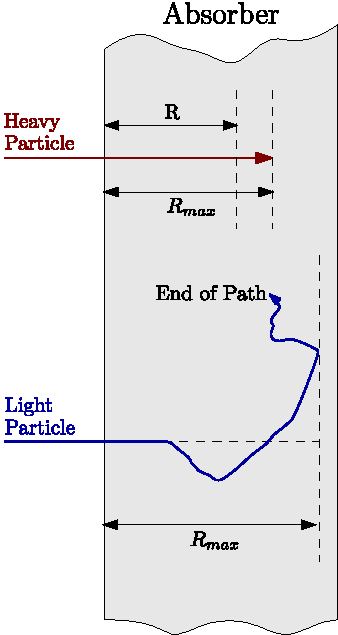
\includegraphics[width=0.30\columnwidth]{RangeVsPath/RangeVsPath.pdf}
    \caption{Schematic diagram of charged particle penetration into absorbing medium. Top: Heavy charged particle. Bottom: Light Charged particle.}
    \label{fig:RangeVsPathLength}
\end{figure}


The range highly depends on the type of particle, its initial energy and on the material through which it passes. Figure \ref{fig:RangeVsPathLength} also illustrates the differences between the path length and range of heavy and light particles. For a heavy particle that losses energy through ionization and atomic excitation, the range (R) can be calculated through the Continuous Slowing Down Approximation (CSDA). This approximation assumes a smooth path, without hard collisions and large-angle scattering. For a particle with an initial energy $E_0$, the CSDA range can be calculated as follows: 

\begin{equation}
    R_{CSDA} = \int_{0}^{E_0} \left( \frac{dE}{dx} \right)^{-1} dE
    \label{eq:rangeCSDA}
\end{equation}

Here the stopping power is considered to be a positive quantity. Some examples of analytical derivations of this equation can be found in \parencite*[][]{ref:CSDA}. The CSDA range for a heavy non-relativistic charged particles, of mass $M_0$ and energy $E_k$, in a given absorber can be written in terms of the proton CSDA range ($R^{p}_{CSDA}$)as follows: 

\begin{equation}
    R_{CSDA}^{M_0} \left( E_K \right)= \frac{1}{Z^2} \left(\frac{M_0}{m_p}\right) R_{CSDA}^{p}\left[ E_K \frac{m_p}{M_0}\right]
\end{equation}

Where $M_p$ is the proton mass and Z is the atomic number of the incident ion. This can be very useful, as the range of protons in a variety of absorbers has been extensively measured. For heavy charged particles, $R_{max} \sim R_{CSDA}$ in all types of absorbing media. 

In the case of light particles, this CSDA approximation is not valid due to the very tortuous path that they experience in the absorbing medium. In this case, the CSDA range can be up to twice the average path for high Z absorbers ($R_{max} = 1/2 R_{CSDA}$). A useful quantity in the case of light particles is called the radiation length ($X_0$), usually measured in $g cm^2$. This gives us a mean distance over which high-energy electron losses all but $1/e$ of its energy by Bremsstrahlung. Different approximations to this value are available in the literature, and each of them includes different degrees of approximations. Some of this expressions can be found in \parencite*[][]{ref:radiationLength}. Just as an example, this would be an expression for high energetic electrons in high Z materials: 

\begin{equation}
    X_0 = \frac{716.405 A}{Z\left(Z+1\right)ln\left(183 Z^{-1/3}\right)}
    \label{eq:radiationlength.}
\end{equation}

\section{Types of Absorbers}

In thin absorbers, only a few collisions of the projectile with the target atoms are likely to happen. Contrarily, in thick absorbers, a projectile makes many collisions and the projectile energy lost by the incident particle is considerable. One can consider a target to be thin when the range of the incident particles is much larger than the thickness of the material ($R(E_k) >> L$). For thin absorbers, the energy loss is small and the stopping power doesn't change much along the length of the material. In this case, the total energy loss in the absorber can be calculated as: 

\begin{equation}
    \Delta E = - \left(\frac{dE}{dx}\right)_{avg} \cdot L
    \label{eq:thinabs}
\end{equation}

In this case, the trajectory of the particle is also assumed to be perfectly linear in the absorber. If the range of the particles in the material is comparable to the thickness or smaller, this approximation is no longer valid, as one would underestimate the real energy deposition in the material. As the energy is lost, the probability of interactions with the absorber material increases as the ionization interaction cross-sections are bigger for smaller energies. The plot representing the specific energy loss along the incident particle track is called the Bragg curve. Figure \ref{fig:Bragg} shows an example of Bragg curve in the case of 3 \si[]{\mega\electronvolt} protons in graphite. 

\begin{figure}[h]
    \centering
    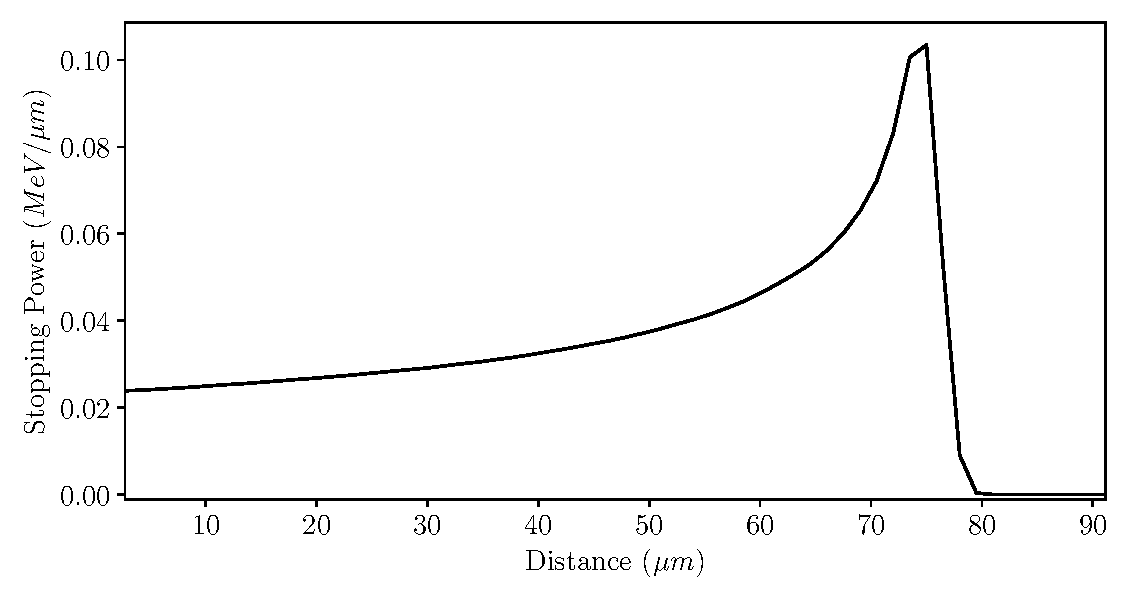
\includegraphics[width=0.7\columnwidth]{Bragg_Graphite/Bragg.pdf}
    \caption{Bragg peak of 3 \si[]{\mega \electronvolt} protons in Graphite. }
    \label{fig:Bragg}
\end{figure}

\section{Secondary Electron Theory}
\label{sec:SEY}
When a particle passes through the interface of a material, it will transfer energy to the
electrons in the medium. Depending on the energy these electrons get, they can be excited
to a higher energy level or gain enough energy to be emitted from the material, this emission
process is known as Secondary Electron Emission (SEE). The SEE phenomenon was already discovered in 1902 by Austin Starke \parencite*[][]{ref:see1} and it has been intensively studied since then. The SEE process can be generally divided into three consecutive steps:

\begin{enumerate}
    \item Generation Process: The minimum energy needed to create a Secondary Electron (SE) is the one required to ionize the atoms in the material. If the incident projectile is an ion containing electrons, these electrons can also be stripped off and produce further ionization. However, if the electrons from the incident ions are scattered off the material, they cannot be counted as secondary electrons. 
    \item Diffusion Process: While the SE travel through the material, they lose energy. This energy loss permits only a very shallow penetration depth of the low-energy electrons. For that reason, SE tends to be a surface phenomenon. 
    \item Emission Process: To be emitted from the surface, the SEs have to overcome the surface barrier potential \parencite*[][]{ref:see2}. The escape process is of particular importance because it determines the final shape of the secondary electron distribution. 
\end{enumerate}

\begin{figure}[h]
    \centering
    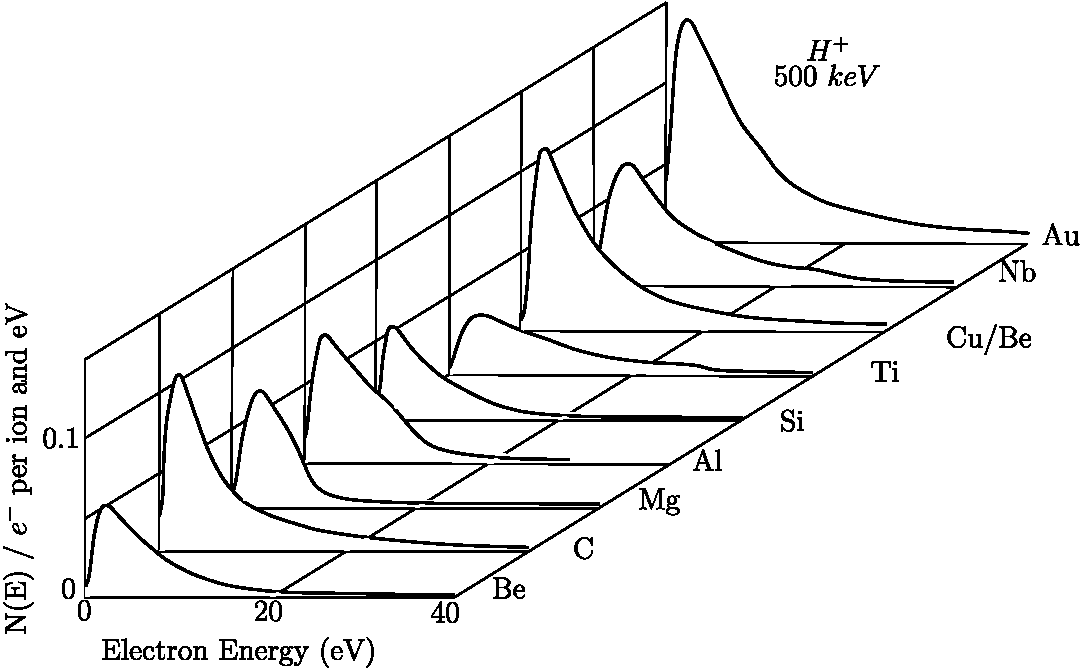
\includegraphics[width=0.9\columnwidth]{SEE_Spectra/SeeSpectra.pdf}
    \caption{Ion induced secondary electron spectra for a variety of metals. Incident ion: Proton 500 \si[]{\kilo \electronvolt}. From \parencite*[][]{ref:SEEspectra} }
    \label{fig:MetalsSE}
\end{figure}

Many experimental measurements on secondary electrons have been done since the discovery of this phenomenon, revealing some commonalities. In the case of SEE from metal surfaces \parencite*[][]{ref:see3},  The energy spectra of SEE peak at about 1-5 eV, showing a quick rise to the peak and then a slow reduction in the intensity. The full width of the peak is around 3-15 \si[]{\electronvolt}. At energies of several tens of \si[]{\electronvolt}, the intensity of the energy spectra is much weakened compared to the maximum peak. One can roughly say that the SE, in general, have an energy $< 50$ \si[]{\electronvolt}. Figure \ref{fig:MetalsSE} shows the spectra of SE emitted from different metals for an incident 500 \si[]{\kilo\electronvolt} proton. 

Not only SE must have an energy that allows them to escape the surface, but their velocity vector when reaching the surface must allow them to escape. In the case of metals and semiconductors, a cosine-type angular distribution of secondary electrons is observed \parencite[][]{ref:angleSemi}. 

The main parameter describing the SEE is the Secondary Emission Yield (SEY), which is the average number of electrons emitted per incident projectile. A semi-empirical treatment of SEY was formulated by E.J. Sternglass in 1957 \parencite*[][]{ref:SEY}. In this formulation, two sources of SE are considered. Firstly, the SE generated by small energy transfers from the incident particles to the target electrons. This first mechanism is the main contributor to the SEY. Secondly, a smaller contribution comes from the SE generated by delta electrons (which will be discussed in the following section). This formulation allows for the following numerical relation: 

\begin{equation}
    SEY = 0.01 L_S \left. \frac{dE}{dx}\right|_{el} \left[ 1+\frac{1}{1+5.4\cdot 10^{-6} E/A_p}\right]
    \label{eq:sey}
\end{equation}
\begin{equation}
    L_S = \left( 3.68\cdot 10^{-17} N Z^{1/3} \right)^{-1}
    \label{eq:LS}
\end{equation}

Here, E and $A_p$ are the kinetic energy and the mass of the projectile. Please notice that the electronic energy loss should be given in (\si[]{\electronvolt/\centi\metre}). $L_{s}$ is the characteristic length, which is of the order of the distance between inelastic collisions, and it is expressed in (\si[]{\centi\metre}). The dependence of the incident particle energy comes with the term $dE/dx$. As we saw previously (\ref{sec:Bethe}), this term is greatly affected by the speed of the incident particle and its nature. 

The Secondary Emission Yield also depends on the angle of incidence of the incident particle. In the theory of Sternglass, the angular dependence is treated as a change in the effective penetration distance $L_{s}$. If the particle impacts under an angle different than normal, the effective track length of the projectile extends by a factor $1/cos(\theta)$. In that case the corresponding SEY would be: 

\begin{equation}
    \frac{SEY(\theta)}{SEY(0)} = \frac{1}{cos(\theta)}
\end{equation}

Experimental values confirm this approximation for incident angles up to $70\deg$. However, in the case of electrons as incident particles, recent measurements show a different angular dependence \parencite*[][]{ref:seyAngleEl}: 

\begin{equation}
    \frac{SEY(\theta)}{SEY(0)} = e^{0.5 \left(1-cos(\theta)\right)}
\end{equation}

Early investigations of SEE already show a dependence of SEE with temperature \parencite*[][]{ref:SeyVsTemp}. The temperature seems to affect the escape probability. An increase in temperature results in increased vibrations of the atoms about their equilibrium position which should reduce $L_{s}$, therefore increasing the Yield. Sternglass gives a rough quantitative hypothesis that goes as follows: 

\begin{equation}
    \frac{L_S (T_1)}{L_S(T_2)} = \frac{1+2.5\cdot 10^{-3}T_1}{1+2.5\cdot 10^{-3}T_2}
\end{equation}

It is important to note that the semiempirical theory of secondary emission is only considered to be accurate for backward emission (projectile entering the target). For the rear face of the target, the secondary emission is difficult to distinguish from the existing $\delta$ rays. On first approximation, we will also consider this formulation to be valid in the rear face assuming that the error due to $\delta$ raw emission can be neglected.  

\section{Delta Rays}

Most frequently, the electrons generated by SE have small energy. However, if the energy transferred to the electron is above a few hundred \si[]{\electronvolt} (up to $T_{max}$), they might be able to generate further ionization on their own. An analytical formulation for the total number of $\delta$-rays produced from charged particle interactions was presented by Rossi in 1952 \parencite*[][]{ref:delta1}, and gives the distribution of $\delta$ rays for incident particles with energy $I \ll T \ll T_{max}$ as follows: 

\begin{equation}
    \frac{d^2N_{\delta}}{dTdx} = \frac{1}{2}Kz^2\frac{Z}{A}\frac{1}{\beta^2}\frac{F(T)}{T^2}
    \label{eq:deltaN}
\end{equation}

Where $Tmax$ is given by equation \ref{eq:tmax}. The factor F is spin-dependent, but it is about unity for $ T \ll  T_{max}$. In order to calculate the total number of generated delta rays per unit of distance, one can integrate the previous equation from an arbitrary lower limit to the maximum energy delta rays can get ($T_{max}$). 

